% !TeX root = ../beamer.tex
\section{Was ist Passiv Radar}

\begin{frame}
    \frametitle{Was ist Radar}

    \begin{columns}
        \begin{column}{0.6\textwidth}
            \begin{itemize}
                \item \textbf{RA}dio \textbf{D}etection and \textbf{R}anging
                \item Messung von \textbf{Entfernung} und \textbf{Geschwindigkeit}
                      \begin{itemize}
                          \item<3-> Zeitversatz \(\tau\)
                          \item<3-> Frequenzversatz \(f_{d}\)
                      \end{itemize}
            \end{itemize}
        \end{column}
        \begin{column}{0.4\textwidth}
            \begin{figure}
                \centering
                \begin{tikzpicture}
                    
\def\tickamp{0.025cm}
\def\tickseg{0.5cm}
\node [label={below:Radar}] (radar) at (0,0) {\Huge\faSatelliteDish};

\node [label={above:Target}] (target) at (3,3) {\Huge\faPlane};

\draw [visible on=<1>,decorate,decoration={expanding waves,angle=6,segment length=3pt},blue!60] (radar) -- node [fg] {\small\contourlength{2pt}\contour{bg}{Pulse}} (target);

\draw [visible on=<2->,decorate,decoration={expanding waves,angle=60,segment length=6pt},red!60] (target) -- node [fg] {\small\contourlength{2pt}\contour{bg}{Echo}} (radar);

                \end{tikzpicture}
            \end{figure}
        \end{column}
    \end{columns}
\end{frame}

\begin{frame}
    \frametitle{Was heißt Passiv?}

    \begin{columns}
        \begin{column}{0.6\textwidth}
            \begin{itemize}
                \item Beleuchtung durch Sender in der \textbf{Umgebung}
                \item Operator hat \textbf{keine Kontrolle} über Beleuchter
                \item Beleuchter und Empfänger sind \textbf{räumlich getrennt}
            \end{itemize}
        \end{column}
        \begin{column}{0.4\textwidth}
            \begin{figure}
                \centering
                \resizebox{\linewidth}{!}{
                    \begin{tikzpicture}
                        \newcommand\drawTopology[4]{
    \coordinate (rx1_coord) at (-2,0);
    \coordinate (tx1_coord) at (2,0);
    \coordinate (target_coord) at (1.25,3);

    \node at (tx1_coord) [text width=0.5cm,text height=1cm] (tx) {};
    \node at (tx1_coord) [antenna,scale=0.5,below=-0.5cm] {};
    \path let \p1=(tx.north west), \p2=(tx.south east), \p3=(tx) in [label={below:Receiver}] ({\x3-0.4cm},\y1) rectangle ({\x3+0.4cm},\y2) node [below] at (\x3,\y2) {Illuminator};

    \node at (rx1_coord) [text width=0.5cm,text height=0.75cm] (rx) {};
    \node at (rx1_coord) [antenna,scale=0.5,below=-0.5cm] {};
    \path let \p1=(tx.north west), \p2=(tx.south east), \p3=(rx) in [label={below:Receiver}] ({\x3-0.4cm},\y1) rectangle ({\x3+0.4cm},\y2) node [below] at (\x3,\y2) {Receiver};

    \node at (target_coord) [label={above:Target}] (target) {\Huge\faPlane};

    \draw [visible on={#1},decorate,decoration={expanding waves,angle=35,segment length=4pt},blue!60] (tx) -- (target);
    \draw [visible on={#2},decorate,decoration={expanding waves,angle=25,segment length=4pt},red!60] (target) -- node [#4] {\small\contourlength{2pt}\contour{#3}{Echo}} (rx);
    \draw [visible on={#1},decorate,decoration={expanding waves,angle=15,segment length=4pt},blue!60] (tx) -- node [#4] {\small\contourlength{2pt}\contour{#3}{Reference}} (rx);
}

                        \drawTopology{<2->}{<3->}{bg}{fg}
                    \end{tikzpicture}
                }
            \end{figure}
        \end{column}
    \end{columns}
\end{frame}

\begin{frame}
    \frametitle{Warum so umständlich?}

    Eigenschaften:
    \begin{itemize}
        \item \textbf{Keine} eigenen \textbf{Abstrahlungen} \faBroadcastTower{}
        \item \textbf{Redundanz} durch bestehende Infrastruktur \faCheckDouble{}
        \item \textbf{Kostengünstiger} \faMoneyBillWave{}
        \item \textbf{Recycling} bestehender Bänder \faRecycle{}
        \item \textbf{Versteckt} operierbar \faEyeSlash{}
    \end{itemize}
\end{frame}

\begin{frame}
    \frametitle{Beleuchtungsquellen (Illuminators of Opportunity)}

    \begin{columns}
        \begin{column}{0.2\textwidth}
            \begin{figure}
                \raggedleft{}
                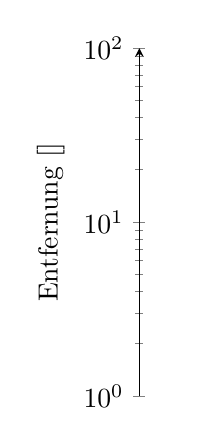
\begin{tikzpicture}
                    \begin{axis}[
                            ymode=log,
                            height=6cm,
                            width=2cm,
                            hide x axis,
                            axis y line=left,
                            ymin=1,
                            ymax=100,
                            ylabel={Entfernung [\si{\kilo\metre}]},
                        ]
                        \addplot [draw=none] {1};
                    \end{axis}
                \end{tikzpicture}
            \end{figure}
        \end{column}
        \begin{column}{0.8\textwidth}
            \begin{itemize}
                \item FM-Radio
                \item DVB-T (Digitales Fernsehen)
                \item DAB (Digitales Radio)
                \item LTE
                \item GSM
                \item WiFi
            \end{itemize}
        \end{column}
    \end{columns}
\end{frame}
